\documentclass[11pt,letterpaper]{article}
\usepackage[lmargin=1in,rmargin=1in,bmargin=1in,tmargin=1in]{geometry}
\usepackage{style/quiz}
\usepackage{style/commands}

\usepackage{textcomp}	% Cent Symbol
\newcommand{\squiggle}{\rightsquigarrow}

% -------------------
% Content
% -------------------
\begin{document}
\thispagestyle{title}

% Quiz 1
\quizsol \textit{True/False}: The product $57(1.08)$ can be interpreted either as both finding 8\% of 57 and increasing 57 by 8\%. \pspace

\sol The statement is \textit{false}. To find a percentage $\%$ of a number $N$, we compute $N \cdot \%_d$, where $\%_d$ is the percentage written as a decimal. But then finding 8\% of 57 is $57(0.08)$, not $57(1.08)$. The product $57(1.08)$ would represent finding 108\% of 57. To find the result of a number $N$ increased or decreased by a percentage $\%$, we compute $N(1 \pm \%_d)$, where $\%_d$ is the percentage written as a decimal, and we choose `$+$' if a percentage increase and `$-$' if a percentage decrease. But then to compute 57 increased by 8\%, we compute $57(1 + 0.08)= 57(1.08)$, as stated in the quiz. Therefore, the quiz statement is false. \pvspace{1.3cm}



% Quiz 2
\quizsol \textit{True/False}: Your GPA after the end of your Freshman year (30~credits) was 3.217. If you took 16 credits in the Fall of your Sophomore year and had a semester GPA of 3.615, then your current GPA is $\frac{30(3.217) + 16(3.615)}{30+16}= \frac{154.35}{46} \approx 3.355$. \pspace

\sol The statement is \textit{true}. To compute ones new GPA, one computes\dots
	\[
	\begin{aligned}
	\text{Overall GPA}&= \dfrac{\text{Previous Credits} \cdot \text{Previous GPA} + \text{Semester Credits} \cdot \text{Semester GPA}}{\text{Total Credits}} \\
	&= \dfrac{30 \cdot 3.217 + 16 \cdot 3.615}{30 + 16} \\
	&= \dfrac{96.51 + 57.84}{30 + 16} \\
	&= \dfrac{154.35}{46} \\
	&\approx 3.355
	\end{aligned}
	\] \pvspace{1cm}



% Quiz 3
\quizsol \textit{True/False}: The distance between the points $(4, 3)$ and $(-1, 6)$ is $\sqrt{(-1 - 4)^2 + (6 - 3)^2}= \sqrt{(-5)^2 + 3^2}= \sqrt{25 + 9}= \sqrt{34} \approx 5.83095$. \pspace

\sol The statement is \textit{true}. The distance between two points $(x, y)$ and $(a, b)$ is $d= \sqrt{(x - a)^2 + (y - b)^2}$. But then taking $(x, y)= (-1, 6)$ and $(a, b)= (4, 3)$, we have\dots
	\[
	d= \sqrt{(-1 - 4)^2 + (6 - 3)^2}= \sqrt{(-5)^2 + 3^2}= \sqrt{25 + 9}= \sqrt{34} \approx 5.83095
	\] \pvspace{1.3cm}



% Quiz 4
\quizsol \textit{True/False}: A 10~ft $\times$ 10~ft $\times$ 20~ft container is filled with 500~ft$^3$ of syrup. More syrup is flowing in at a rate of 40~ft$^3$ per minute. Because the volume is $10 \cdot 10 \cdot 20= 2000 \text{ ft}^3$, the time it will take to fill the container is $t= \frac{2000 \text{ ft}^3}{40 \text{ ft}^3/\text{min}}= 50 \text{ min}$. \pspace

\sol The statement is \textit{false}. We know that the net change is given by $C= rt$, where $C$ is the net change, $r$ is the rate, and $t$ is the time. But then $t= \frac{C}{r}$. We know that the volume of the container is $V= \ell wh= 10 \text{ ft} \cdot 10 \text{ ft} \cdot 20 \text{ ft}= 2000 \text{ ft}^3$. Because the container already contains $500 \text{ ft}^3$ of syrup, the amount of space left in the container is $2000 \text{ ft}^3 - 500 \text{ ft}^3= 1500 \text{ ft}^3$. Because the syrup is flowing in at a rate of $r= 40 \text{ ft}^3/\text{min}$, the amount of time it will take to fill the (remainder of) the container is $t= \frac{1500 \text{ ft}^3}{40 \text{ ft}^3/\text{min}}= 37.5 \text{ min}$. We can see that the given time was the time it would take to fill the entire container from an empty state. \pvspace{1.3cm}



% Quiz 5
\quizsol \textit{True/False}: Alice and Bob and start at the same location. Alice travels north at 3~mph and Bob travels east at 4~mph. Two hours later, Alice has traveled $3 \text{ mph} \cdot 2 \text{ hr}= 6 \text{ mi}$, Bob has traveled $4 \text{ mph} \cdot 2 \text{ hr}= 8 \text{ mi}$, and Alice and Bob are $6 \text{ mi} + 8 \text{ mi}= 14 \text{ mi}$ apart. \pspace

\sol The statement is \textit{false}. Alice and Bob start at the same point. Alice travels north at 3~mph and Bob travels east at 4~mph. We know that $d= rt$, where $d$ is the distance, $r$ is the travel rate, and $t$ is the time. We know Alice travels a distance of $d= 3 \text{ mph} \cdot 2= 6 \text{ mi}$ north. Bob travels a distance of $d= 4 \text{ mph} \cdot 2= 8 \text{ mi}$. We can diagram this scenario out:
	\[
	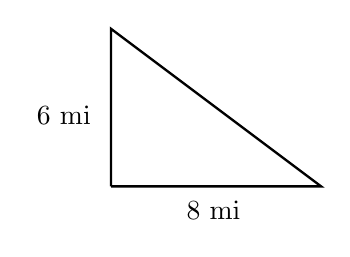
\begin{tikzpicture}
	\draw[line width=0.03cm] (0,0) -- (0,3/1.5) -- (4/1.5,0) -- (0,0);
	\node at (-0.6,0.9) {6~mi};
	\node at (1.3,-0.3) {8~mi};
	\end{tikzpicture}
	\]
Clearly, this is a right triangle. For right triangles, we know that $c^2= a^2 + b^2$, where $a, b$ are legs of the right triangle and $c$ is the hypotenuse. The distance between Alice and Bob is the length of the hypotenuse. But then\dots
	\[
	\begin{gathered}
	c^2= a^2 + b^2 \\
	c^2= (6 \text{ mi})^2 + (8 \text{ mi})^2 \\
	c^2= 36 \text{ mi}^2 + 64 \text{ mi}^2 \\
	c^2= 100 \text{ mi}^2 \\
	c= \sqrt{100 \text{ mi}^2} \\
	c= 10 \text{ mi}
	\end{gathered}
	\]
Therefore, Alice and Bob are 10~miles apart. One cannot simply add/subtract distances unless all the distances lie along the same line---but one need take care of the direction along the line. \pvspace{1.3cm}

 

% Quiz 6
\quizsol \textit{True/False}: If $f(x)= 5x - 4$ and $g(x)= 6x$, then $(f \circ g)(2)= f(2) \cdot g(2)= 6 \cdot 12= 72$. \pspace

\sol The statement is \textit{false}. We know that $(f \circ g)(2)= f \big( g(2) \big)$. We have $g(2)= 6(2)= 12$. But then $f \big( g(2) \big)= f(12)$. Finally, $f(12)= 5(12) - 4= 60 - 4= 56$. Therefore, $(f \circ g)(2)= 56$. The statement finds the value of $(fg)(2)= 72$, whereas the given function, $f \circ g$, is function composition. 

 

\newpage



% Quiz 7
\quizsol \textit{True/False}: The function $f(x)= \dfrac{x + 1}{x - 3}$ is linear. \pspace

\sol The statement is \textit{false}. A function is linear if it can be written in the form $y= mx + b$ for some $m, b$. While the numerator and denominator are linear, the function itself is not linear. We know the graph of a linear function is a line. We can see from the graph of $f(x)$ that $f(x)$ is not linear. 
	\[
	\fbox{
	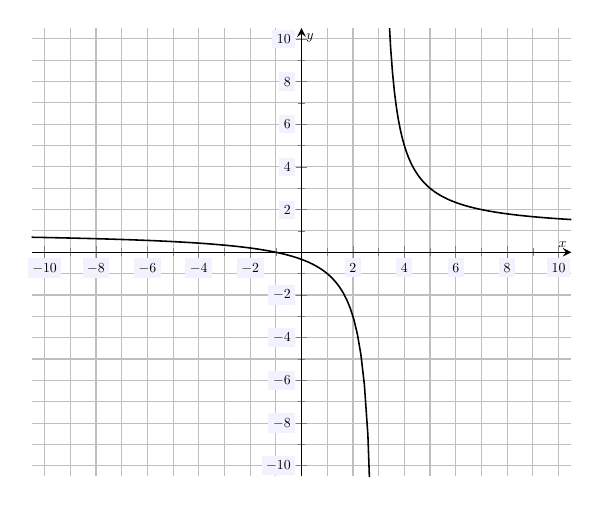
\begin{tikzpicture}[scale=1,every node/.style={scale=0.5}]
	\begin{axis}[
	grid=both,
	axis lines=middle,
	ticklabel style={fill=blue!5!white},
	xmin= -10.5, xmax=10.5,
	ymin= -10.5, ymax=10.5,
	xtick={-10,-8,-6,-4,-2,0,2,4,6,8,10},
	ytick={-10,-8,-6,-4,-2,0,2,4,6,8,10},
	minor tick = {-10,-9,...,10},
	xlabel=\(x\),ylabel=\(y\),
	]
	\addplot[line width= 0.02cm,samples=100,domain= -10.5:2.99] ({x},{(x+1)/(x - 3)});
	\addplot[line width= 0.02cm,samples=100,domain= 3.01:10.5] ({x},{(x+1)/(x - 3)});
	\end{axis}
	\end{tikzpicture}
	}
	\] \pvspace{1.3cm}



% Quiz 8
\quizsol \textit{True/False}: In `real-life', exponential growth is not sustainable and `most often' logistic models have to be used. \pspace

\sol The statement is \textit{true}. Take an initial population of one that grows by 0.1\% per year, every year. Then we know the population after $t$ years is given by $1(1 + 0.001)^t= 1(1.001)^t= 1.001^t$, which is clearly an exponential function. Even with this small initial population and tiny growth rate, after 15,000~years, the population is $1.001^{15000} \approx 3,\!244,\!607.7$. Of course, even assuming an initial starting population of 500 and an annual increase of 5\% per year, after 300~years, the population would be $500(1 + 0.05)^{300}= 500(1.05)^{300} \approx 1,\!136,\!998,\!064.3$. This type of growth is not sustainable. As the population increases, resources decrease and the environment cannot sustain the population growth. The growth tapers off and becomes logistic. Logistic models include not only the initial exponential growth, but also the `tapering off' of the growth rate as well. \pvspace{1.3cm}



% Quiz 9
\quizsol \textit{True/False}: The current CPI is $307.789$ and if next year it is $318.438$, then the inflation rate was $\frac{318.438}{307.789}= 1.0346$; hence, the inflation rate from this year to next year would be 3.46\%. \pspace

\sol The statement is \textit{true}. If the inflation rate is $r_d$, where $r_d$ is the inflation rate written as a decimal, $P$ is the current CPI, and $F$ is next year's CPI, then we know that $F= P(1 + r)$; that is, the next year's CPI is the current CPI increased by $r$. But then 
	\[
	\begin{gathered}
	F= P(1 + r) \\
	318.438= 307.789(1 + r) \\
	1.034598377= 1 + r \\
	r= 0.034598377
	\end{gathered}
	\]
Therefore, the inflation rate from this year to next year is 3.46\%. Alternatively, we know that the inflation rate is given by\dots
	\[
	\text{Inflation Rate}= \dfrac{\text{New CPI}}{\text{Old CPI}} - 1= \dfrac{318.438}{307.789} - 1= 1.034598377 - 1= 0.034598377 \squiggle 3.46\%
	\] \pvspace{1.3cm}



% Quiz 10
\quizsol \textit{True/False}: If you invest \$250 at 4.8\% annual interest, compounded quarterly for 8 years, then the investment is worth $\$250 \left(1 + \dfrac{0.048}{4} \right)^8 \approx \$275.03$. \pspace

\sol The statement is \textit{false}. We know that if a principal amount, $P$, is invested at an annual interest rate, $r$, compounded $k$ times per year, then the value after $t$~years is given by $F= P \left(1 + \frac{r}{k} \right)^{kt}$. Here we have a principal of $P= \$250$ and an annual interest rate of $r= 0.048$, compounded $k= 4$~times per year. The amount after 8~years is then\dots
	\[
	F= P \left(1 + \dfrac{r}{k} \right)^{kt}= \$250 \left(1 + \dfrac{0.048}{4} \right)^{4 \cdot 8}= \$250 (1.012)^{32}= \$250 (1.4647934865) \approx \$366.20
	\]
The given expression has power 8 rather than the total number of compounds $4 \cdot 8= 32$. \pvspace{1.3cm}



% Quiz 11
\quizsol \textit{True/False}: A series of equal payments at equal time intervals is an annuity. \pspace

\sol The statement is \textit{true}. An annuity is a series of equal payments over equal time periods. If the payments are the end of a payment period, this is an annuity immediate or an ordinary annuity. If the payments are made at the start of a payment period, this is an annuity due. If the number of interest compounds per year is equal to the number of payments per year, then it is a simple annuity. If not, then it is a general annuity. \pvspace{1.3cm}



% Quiz 12
\quizsol \textit{True/False}: One will always make more interest compounding continuously than compounding $k$ times per year at the same interest rate, no matter the value for $k$. \pspace

\sol The statement is \textit{true}. We know that the more one compounds, the more interest one receives---even if the interest is small, subsequent interest received is on a larger amount. Therefore, a greater the number of compounds results in a greater amount of money in the same amount of time. To compound continuously means to compound interest infinitely often, i.e. the limit as the number of compounds tends to infinity. But then at the same level of interest, $r$, compounding continuously will always result in more interest for any number of compounds, $k$, per year. One can prove this mathematically, essentially following from this argument: if $x, r, P$ are real numbers and $r, P > 0$, then 
	\[
	P \left(1 + \dfrac{r}{k} \right)^{kt} \leq Pe^{kt \cdot \frac{r}{k}}= Pe^{rt}
	\]
But a full proof of this fact is beyond our scope. \pvspace{1.3cm}



\newpage



% Quiz 13
\quizsol \textit{True/False}: The amount you would have to invest at 1.3\% annual interest, compounded continuously to have \$8,000 in 5 years is $\frac{\$8000}{e^{0.13 \cdot 5}} \approx \$4176.37$. \pspace

\sol The statement is \textit{false}. The future value, $F$, of a principal $P$ earns interest at an annual interest rate $r$, compounded continuously for $t$ years is given by $F= Pe^{rt}$. But then the amount needed to invest, a principal $P$, to accumulate to a value $F$ in $t$ years if $P$ earns an annual interest $r$, compounded continuously is given by $P= \frac{F}{e^{rt}}$. But then the amount one would have to invest at 1.3\% annual interest, compounded continuously to have \$8,000 in 5 years is 
	\[
	P= \dfrac{F}{e^{rt}}= \dfrac{\$8,\!000}{e^{0.013 \cdot 5}}= \dfrac{\$8,\!000}{e^{0.065}}= \dfrac{\$8,\!000}{1.067159024} \approx \$7,\!496.54
	\]
The proposed solution uses an annual interest rate of 13\%, rather than 1.3\%. \pvspace{1.3cm}



% Quiz 14
\quizsol \textit{True/False}: Because artificial intelligence algorithms execute code to learn from data, they are free from bias. \pspace

\sol The statement is \textit{false}. We saw in \textit{Coded Bias} that modern machine learning techniques teaches computer to learn from data. But what computers `learn' is only as good as the data fed to these machines. If the data contains bias---intentional or unintentional---the computer algorithms themselves reflect these biases. \pvspace{1.3cm}



% Quiz 15
\quizsol \textit{True/False}: You have 5 coins in your pocket: two dimes and three nickels. If you choose two coins from your pocket, one after the other, the probability of getting 20\textcent\ is $\frac{2}{5} \cdot \frac{2}{5}= \frac{4}{25} \approx 0.16$. \pspace

\sol The statement is \textit{false}. If $A, B$ are events, then one can only compute $P(A \text{ and } B)$ using $P(A \text{ and } B)= P(A) \cdot P(B)$ only if $A$ and $B$ are independent, i.e. if the occurrence or non-occurence of $A$ or $B$ does not chance the probability of $B$ or $A$, respectfully. To pull 20\textcent\ from one's pocket, one would need to pull two dimes---one after the other. The probability of pulling the first dime is $\frac{2}{5}$. However, after pulling this dime, the probability of pulling the next dime is $\frac{1}{4}$---because there is one less dime and one less coin overall. Observe the probability of pulling the first dime affected the probability of pulling the next dime, i.e. these events are not independent. The probability is then $\frac{2}{5} \cdot \frac{1}{4}= \frac{1}{10} \approx 0.10$. We can see this directly from the more general formula of computing the probability of two events occurring simultaneously---$P(A \text{ and } B)= P(A) \cdot P(B)$:
	\[
	P(\text{two dimes})= P(\text{dime and dime})= P(\text{dime}) P( \text{dime} \;|\; \text{dime})= \dfrac{2}{5} \cdot \dfrac{1}{4}= \dfrac{1}{10} \approx 0.10
	\] \pvspace{1.3cm}



% Quiz 16
\quizsol \textit{True/False}: If $A$ and $B$ are independent events, then $P(A)= P(A \;|\; B)$ and $P(B)= P(B \;|\; A)$. \pspace

\sol The statement is \textit{true}. If $A$ and $B$ are independent, then the occurrence or non-occurrence of $A$ does not affect the probability of $B$ and vice versa. We know that $P(A \;|\; B)$ is the probability of $A$ given that $B$ occurs. But if $A, B$ are independent, then $B$'s occurrence does not change the probability that $A$ occurs. But then $P(A \;|\; B)= P(A)$. Similarly, $P(B \;|\; A)= P(B)$. We can see this directly from the definition of $A$ and $B$ being independent: $P(A \text{ and } B)= P(A) \cdot P(B)$. If this is true, then\dots
	\[
	P(A \;|\; B)= \dfrac{P(A \text{ and } B)}{P(B)}= \dfrac{P(A) P(B)}{P(B)}= P(A), \qquad P(B \;|\; A)= \dfrac{P(B \text{ and } A)}{P(A)}= \dfrac{P(B) P(A)}{P(A)}= P(B)
	\] \pvspace{1.3cm}



% Quiz 17
\quizsol \textit{True/False}: There is no difference between a random sample and a simple random sample. \pspace

\sol The statement is \textit{false}. A random sample is a sample in which every \textit{individual} is equally likely to be a part of the sample as any other individual. A simple random sample is a sample in which any \textit{group} of individuals is equally likely to appear as any other group of individuals. Depending on the method of selecting a sample, any sample can be both a random sample and a simple random sample, a random sample but not a simple random sample, or neither a random sample nor a simple random sample. \pvspace{1.3cm}



% Quiz 18
\quizsol \textit{True/False}: The standard deviation is a measurement of variability about the median. Moreover, the greater the standard deviation, the more `spread out' the data values are. \pspace

\sol The statement is \textit{false}. When examining data, two characteristics one is often interested in are the `center' of the data and the `spread' of the data. We examined several notions of `center': midrange, median, and mean. To each notion of center, one has a notion of `spread.' For the midrange, median, and mean, these are the range, IQR, and standard deviation, respectively. Therefore, the standard deviation is a measurement of variability (or `spread') about the \textit{mean}---not the median. The first statement of the quiz is false. However, because standard deviation is a measurement of spread, larger standard deviations result in largest spread (about the mean). \pvspace{1.3cm}



% Quiz 19
\quizsol \textit{True/False}: For a normal distribution $N(100, 10)$ with a random variable $X$ drawn from this distribution, $P(X > 110)= P(X < 90)$. \pspace

\sol The statement is \textit{true}. We know that a normal distribution is symmetric. We know that $z_{110}= \frac{110 - 100}{10}= \frac{10}{10}= 1$, so that $100$ is one standard deviation above the mean. We want the area under the normal distribution to the right of $110$ because we want $P(X > 110)$. Furthermore, we know that $z_{90}= \frac{90 - 100}{10}= \frac{-10}{10}= -1$, so that $90$ is one standard deviation above the mean. We want the area under the normal distribution to the left of $90$ because we want $P(X < 90)$. But then we want the area under the normal distribution to the left of one standard deviation below the mean and the area under the normal distribution to the right of one standard deviation above the mean. Because the normal distribution is symmetric, these must be the same. One can also compute directly that $z_{110}= 1 \squiggle 0.8413$ and $z_{90}= -1 \squiggle 0.1587$. But then $P(X > 110)= 1 - 0.8413= 0.1587$ and $P(X < 90)= 0.1587$, so that $P(X > 110)= P(X < 90)$. 



\newpage



% Quiz 20
\quizsol \textit{True/False}: For a fixed confidence level, the larger the sample size, the less the margin of error in a confidence interval. \pspace

\sol The statement is \textit{true}. Intuitively, this is obvious. If one samples a single individual, one has nearly no information about the possibilities about the true mean, $\mu$, for the population. If one samples the \textit{entire} population, you know the mean $\mu$ exactly. As the sample size grows from $n= 1$ to the entire population, the amount of uncertainty about the true value for $\mu$, i.e. the error, must decrease. We can see this directly from the construction of the confidence interval. For a fixed confidence level $C$, we obtain a fixed $z^*$-value. The confidence interval is constructed from the two numbers $\overline{x} \pm z^* \frac{\sigma}{\sqrt{n}}$, where $\overline{x}$ is the sample mean, $\sigma$ is the population standard deviation, and $n$ is the sample size. The term $z^* \frac{\sigma}{\sqrt{n}}$ is the margin of error. The larger the value of $n$, the larger the value of $\sqrt{n}$. But as $\sqrt{n}$ gets larger, $\frac{1}{\sqrt{n}}$ gets smaller. But then as $n$ gets larger, $z^* \sigma \cdot \frac{1}{\sqrt{n}}= z^* \frac{\sigma}{\sqrt{n}}$ gets smaller, i.e. the margin of error gets smaller. Therefore, the larger the sample size, the less the margin of error in a confidence interval. 


\end{document}